\documentclass[letterpaper]{article} 
\usepackage[left = 0.5in, right = 0.5in, top = 0.9in, bottom = 0.9in]{geometry}
\usepackage{enumitem}
\usepackage{multicol}
\usepackage[spanish]{babel}
\usepackage[utf8]{inputenc}

\usepackage{amsmath,amssymb,amsthm}
\usepackage{tikz-cd}
\usepackage{mathrsfs}
\usepackage[bbgreekl]{mathbbol}
\usepackage{dsfont}
\usepackage{graphicx}
\graphicspath{{img/}}

\newcommand{\op}{\operatorname}
\newcommand{\Op}{^{\op{op}}}
\newcommand{\scc}{\mathscr C}
\newcommand{\scd}{\mathscr D}
\newcommand{\sce}{\mathscr E}
\newcommand{\sci}{\mathscr I}
\newcommand{\scj}{\mathscr J}
\newcommand{\scx}{\mathscr X}
\newcommand{\var}{\mathrm{Var}}
\newcommand{\Id}{\operatorname{Id}}
\newcommand{\N}{\mathbb N}
\newcommand{\Z}{\mathbb Z}
\newcommand{\Q}{\mathbb{Q}}
\newcommand{\I}{\mathbb{I}}
\newcommand{\R}{\mathbb{R}}
\newcommand{\C}{\mathbb{C}}
\newcommand{\F}{\mathcal{F}}
\newcommand{\G}{\mathcal{G}}
\newcommand{\B}{\mathcal{B}}
\newcommand{\abs}[1]{\left\lvert #1 \right\rvert}
\newcommand{\inv}{^{-1}}
\renewcommand{\to}{\rightarrow}
\newcommand{\ent}{\Longrightarrow}
\newcommand{\E}{\mathbb{E}}
\renewcommand{\P}{\mathbb{P}}
\newcommand{\1}{\mathds{1}}
\renewcommand{\qedsymbol}{$\blacksquare$}

\theoremstyle{definition}
\newtheorem{dfn}{Definición}
\theoremstyle{definition}
\newtheorem{teo}{Teorema}
\theoremstyle{definition}
\newtheorem{cor}{Corolario}
\theoremstyle{definition}
\newtheorem{prop}{Proposición}
\theoremstyle{definition}
\newtheorem{obs}{Observación}


\title{\textbf{Cómputo Científico\\Tarea 4\\Cálculo de eigenvalores}}
\author{Iván Irving Rosas Domínguez}
\date{\today}

\DeclareSymbolFontAlphabet{\mathbbm}{bbold}
\DeclareSymbolFontAlphabet{\mathbb}{AMSb}
\DeclareMathSymbol\bbDelta  \mathord{bbold}{"01}

\begin{document}
\maketitle

%\begin{abstract}
%\end{abstract}

\begin{enumerate}
    \item[\textbf{1.}] Dado el siguiente:
    \begin{teo}[Gershgorin]
        Dada una matriz $A=(a_{ij})$ de $m\times m$, cada eigenvalor de $A$ está en al menos
        uno de los discos en el plano complejo con centro en $a_{ii}$ y radio $\sum_{j\neq i}|a_{ij}|$. 
        Además, si $n$ de estos discos forman un dominio conexo, disjunto de los otros $m-n$ discos, 
        entonces hay exactamente $n$ eigenvalores en ese dominio.
    \end{teo}
    Deduce estimaciones de los eigenvalores de 
\[
    \begin{pmatrix}
    8 & 1 & 0\\
    1 & 4 & \epsilon\\
    0 & \epsilon & 1\\    
    \end{pmatrix}
    \]
    con $|\epsilon|<1$.\\

    \textbf{Solución:} dado el teorema anterior, procedemos a calcular los discos de Gershgorin para $i=1,2,3$.
    \begin{enumerate}
        \item $D_{1}=\left\{z\in \C : |z-8|\leq 1+0\right\}=D_{1}(8)$, el disco complejo de radio 1 con 
        centro en 8.
        \item $D_{2}=\left\{z\in\C : |z-4|\leq 1+\epsilon\right\}=D_{1+\epsilon}(4)$, el disco complejo de 
        radio 1 con centro en 4.
        \item $D_{3}=\left\{z\in \C : |z-1|\leq \epsilon\right\}=D_{\epsilon}(1)$, el disco complejo de radio
        $\epsilon$ con centro en 1.
    \end{enumerate}
    No obstante, dado que la matriz es simétrica y suponiendo que $\varepsilon\in \R$, entonces tiene entradas reales, así que sus eigenvalores son reales, por lo que
    podemos descartar los discos complejos y hablar de intervalos en la recta real. Luego, los Discos de Gershgorin están dados por 
    \begin{enumerate}
        \item $D_{1}=[7,9]$, la bola cerrada con centro en 8 y radio 1,
        \item $D_{2}=[3-\epsilon,5+\epsilon]$, la bola cerrada con centro en 4 y radio $1+\epsilon$,
        \item $D_{3}=[1-\varepsilon,1+\varepsilon]$, la bola cerrada con centro en 1 y radio $\epsilon$,
    \end{enumerate}
    \item[\textbf{2.}] Implementa la iteración $QR$ con shift. Aplícala a la matriz $A$ del Ejercicio 1 con 
    $\epsilon=10^{-N}$ para $N=1,3,4,5$.\\

    \textbf{Solución:} para este ejercicio recurrimos al script de Python llamado \textit{Ejercicio 2-5}.
    En él, se construye el algoritmo \textit{QRshift}, el cual implementa justamente el algoritmo QR con shift
    para llevar a una matriz $A$ a una matriz cuya diagonal posea los eigenvalores de la misma (siempre que esta sea 
    diagonalizable). La función tiene dos argumentos, siendo el primero de ellos la matriz 
    a la cual se le van a extraer los eigenvalores, y el segundo es el número de iteraciones 
    que se quieren realizar en el algoritmo.
    
    Dado que las entradas de la matriz debajo de la diagonal convergen a 0, un alto número 
    de iteraciones puede producir un error, ya que se excede el tamaño mínimo manejable por la computadora.\\
    
    El algoritmo tiene la posibilidad de regresar 3 objetos. El primero de ellos contiene 
    a la matriz $A$ que justamente resulta del algoritmo. El segundo regresa la matriz $Q$ de la última
    iteración y que teóricamente converge a la matriz de eigenvectores de $A$. El tercero corresponde al 
    vector de eigenvalores de $A$.
    \newline

    Luego de cargar las cuatro matrices del ejercicio 1 e implementar el algoritmo con cada una, 
    se obtienen los resultados de la figura 1.
    \begin{figure}[h!]
        \centering
        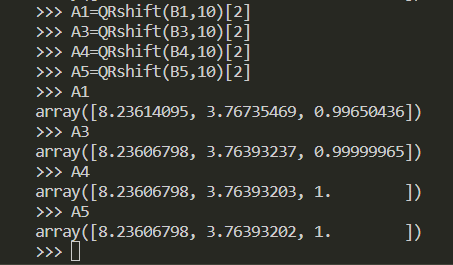
\includegraphics[width=0.6\linewidth]{1.png}
        \caption{Vector de eigenvalores de cada una de las cuatro matrices correspondientes a $\varepsilon=10^{-N}, N=1,3,4,5.$}
    \end{figure} 
    Observamos que en efecto conforme $\varepsilon$ se hace más pequeño, el vector de los eigenvalores converge a $(8.23606798,\ 3.76393202,\ 1.)$,
    los cuales son justamente los eigenvalores de la matriz
    \[
        X=\begin{pmatrix}
        8 & 1 & 0\\
        1 & 4 & 0\\
        0 & 0 & 1\\    
        \end{pmatrix},
        \]
        como se puede corroborar en la figura 2 que contiene los eigenvalores de la matriz anterior y que fueron hallados usando 
        la función $scipy.linalg.eigvals$. 
        \begin{figure}[h!]
            \centering
            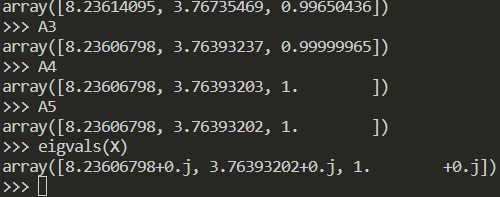
\includegraphics[width=0.6\linewidth]{2.png}
            \caption{Vector de eigenvalores de la matriz X. Los resultados coinciden con los del algoritmo QR haciendo $\varepsilon$ 
            pequeño, y con las estimaciones de los discos de Gershgorin}
        \end{figure} 

    \item[\textbf{3.}]Determina todos los eigenvalores y eigenvectores de una matriz de Householder.
    Aseguramos que los eigenvalores de una matriz de Householder son solo 1 y -1.
    \begin{proof} 
       Por definición, una matriz de Householder está dada por $P=I_n-2vv^*$, donde $v$ es un vector de norma 1 que es normal 
       a un hiperplano generado por $n-1$ vectores $v_n,...,v_n$ en $\R^n$. Notemos que si realizamos $Pv_i, i\in \{2,...,n\}$,
       se tiene que
       \[
       Pv_i=I_nv_i-2vv^*v_i=v_i-2v(0)=v_i, 
       \]  
       ya que $v^*v_i=0$ pues $v$ es ortogonal a $v_i$, con $i\in \{2,...,n\}$. Por lo tanto, tenemos que para cualquier 
       $u\in <v_2,...,v_n>$, $Pu=u$, ya que justamente la propiedad anterior se cumple para la base. Luego, $1$ es un eigenvalor
       de $P$ y además, $v_2,...,v_n$ son eigenvectores asociados al eigenvalor 1. Nótese ahora que 
       \[
        Pv=I_nv-2vv^*v=v-2v(v^*v)=v-2v(1)=-v,
       \]
       ya que $v$ es ortonormal y por lo tanto $v^*v=\|v\|^2=1$. Luego, para cualquier $u\in <v>$, se tiene que $Pu=-u$ por la misma 
       propiedad universal de las bases. Concluimos que $-1$ también es un eigenvalor de $P$ y que $v$ se puede considerar 
       un eigenvector asociado a dicho valor.\\

       Denotando por $v_1:=v$, tenemos que $1$ y $-1$ son los eigenvalores de una matriz de Householder asociados a 
       los vectores $v_1,...,v_n$ que forman una base de $R^n$.
     \end{proof}
    \item[\textbf{4.}]Demuestra que no es posible construir la transformación de similaridad del Teorema
    de Schur con un número finito de transformaciones de similaridad de Householder.\\

    \textbf{Solución:} el teorema de Schur nos dice que si tenemos una matriz $A\in M_n(\C)$, entonces existen $Q$ matriz unitaria
    y $U$ una matriz triangular superior tales que 
    \[
    A=Q^*UQ,    
    \]
    y además, las entradas de la diagonal de $U$ son los eigenvalores de la matriz $A$. Por otro lado, sabemos que si $n\geq5$, entonces 
    \[
    det(A-\lambda I_n),
    \]
    el polinomio característico de $A$ que tiene por raíces a los eigenvalores de la matriz $A$ no tiene una fórmula  
    para resolverse en términos de operaciones que involucren sumas, multiplicaciones y potencias, lo cual
    se deduce del célebre teorema de Abel-Ruffini.\\

    Finalmente, las transformaciones de similaridad de Householder son transformaciones lineales, las cuales 
    están descritas justamente por las matrices de Householder. Por lo tanto, si en un número finito de 
    transformaciones de Householder se pudiera obtener la descomposición del teorema de Schur, entonces tendríamos una 
    fórmula para solución de la ecuación de grado 5 o superior, lo cual es imposible.\\

    Dicho de manera más precisa, si $P_1,...,P_m$ son una sucesión finita de transformaciones de Householder codificadas 
    en las $m$ matrices (de Householder) anteriores, de tal forma que  
    \[
        P_m\cdot P_{m-1}\cdot...\cdot P_1 A=Q^*U^*Q,
    \]
    donde $Q^*UQ$ es la descomposición de $A$ del teorema de Schur, entonces se tendría una fórmula para hallar las soluciones del
    polinomio característico, de grado mayor o igual a 5, de $A$. A saber, la fórmula estaría dada por 
    \[
    \lambda_k=U_{kk}=(QP_m\cdot P_{m-1}\cdot...\cdot P_1 AQ^*)=\sum_{k,j,i_1...,i_{m-1},i_m,l,k}^{n}Q_{kj}P_{m,ki_1}P_{m-1,i_1i_2}\cdot...\cdot P_{1,i_{m-1}i_m}A_{i_ml}(Q^*)_{lk},    
    \]
    pero esto contradice lo que hemos dicho. La afirmación del ejercicio se sigue.
    \item[\textbf{5.}]¿Qué pasa si aplicas la iteración $QR$ sin shift a una matriz ortogonal?\\
    
    \textbf{Solución:} sabemos que la descomposición QR es única salvo cambios de signo (ver Trefethen, Bau), por lo que si una matriz $A$ es ortogonal, entonces podemos verla como
    $A=A\cdot I_n=Q\cdot R $, donde $A=Q$ y $I_n=R$. Luego, al aplicar el algoritmo QR a la matriz $A$ ortogonal, entonces $A=QR=A\cdot I_n \ent RQ=I_n\dot A=A$, 
    de manera que la matriz se queda inalterada. Esto se puede apreciar computacionalmente en la figura 3. El código está al final del script \textit{Ejercicio 2-5}.
    La implementación es exactamente la misma que la hecha en el ejercicio 2 salvo que no se utiliza un shift en el algoritmo.
    \begin{figure}[h!]
        \centering
        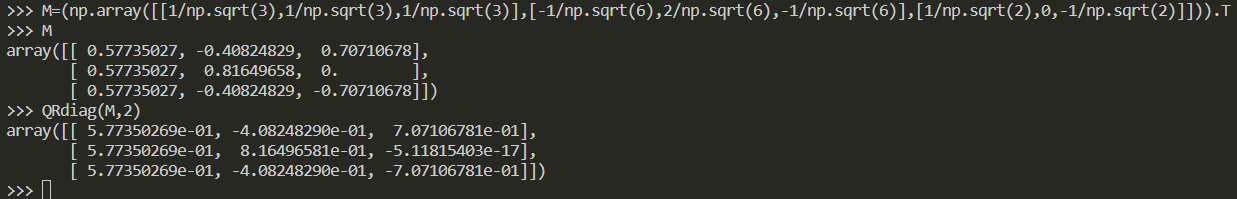
\includegraphics[width=0.9\linewidth]{3.png}
        \caption{Corroboración de que una matriz ortogonal queda inalterada bajo el algoritmo QR.}
    \end{figure}
\end{enumerate}

\end{document}